\documentclass[a4paper, 12pt, oneside]{book}

\usepackage{graphicx}
\usepackage{geometry}
\geometry{
    a4paper,
    left=20mm,
    right=20mm,
    top=20mm,
    bottom=20mm,
}

%permet d'appeler le titre, l'autheur et la date de la thèse
\usepackage{titling} 

\title{Le titre de la thèse d'exercice}
\author{Nom de l'auteur}
\date{01/01/2023}


% Langue
\usepackage[cyr]{aeguill}
% Ce package permet d’afficher et de prendre correctement en charge ces caractères accentués
\usepackage[T1]{fontenc}
\usepackage{xspace}
% Ce package permet d'obtenir des documents en plusieurs langues, en respectant les typographies nationales, en affichant automatiquement les titres
\usepackage[english,french]{babel}
% Ce package permet d'avoir les césures
\usepackage{hyphenat}
%Permet de metre entre guillemets facilement (utiliser le format : \g{Texte exemple})
\newcommand{\g}[1]{\og\,#1\,\fg}
% Ce package permet d'avoir des liens hypertextes dans le document
\usepackage[hidelinks, breaklinks]{hyperref} 

%%%%%%%%%%%%%%%%%%%%%%%%%%%%%%
% Gestion des acronymes      %
%%%%%%%%%%%%%%%%%%%%%%%%%%%%%%
\usepackage{acronym}

%%%%%%%%%%%%%%%%%%%%%%%%%%%%%%
% Gestion bibliographie      %
%%%%%%%%%%%%%%%%%%%%%%%%%%%%%%
\usepackage[autostyle]{csquotes}
% 0. Norme ieee
%\usepackage[backend=biber,style=ieee]{biblatex}

% 1. Norme système Vancouver
% Tricks pour passer le système Vancouver en Français
\usepackage[style=vancouver, citestyle=numeric, sorting=none, dateabbrev=false]{biblatex} 
\DeclareFieldFormat{labelnumberwidth}{\mkbibbrackets{#1}}

\DeclareFieldFormat{date}{#1}
\DefineBibliographyStrings{french}{
  urlseen = {cité le},
  urlfrom = {disponible sur :},
}
\DeclareFieldFormat{url}{\bibstring{urlfrom}\addcolon\space\url{#1}}
\DeclareFieldFormat{urldate}{\bibstring{urlseen}\space#1}
\renewbibmacro*{url+urldate}{%
  \usebibmacro{urldate}%
  \newunit
  \usebibmacro{url}}
% Fin style vancouver français

% Déclaration du fichier de la bibliographie (.bib)
\addbibresource{references/bibliographie.bib}

% Ce package permet de mettre en place des zones encadrées (cf. page de garde)
\usepackage{mdframed} 
\newmdenv[
  skipabove=\topsep,
  skipbelow=\topsep,
]{boxed}


% Ne pas mettre en place d'indentation dans les nouveaux paragraphes
\setlength{\parindent}{0pt}

% Code facile pour écrire des lignes en pointillées
\usepackage{multido}
\newcommand{\Pointilles}[1]{%
  \par\nobreak
  \noindent\rule{0pt}{1.5\baselineskip}
  \multido{}{#1}{\noindent\makebox[\linewidth]{\dotfill}\endgraf}
  \bigskip
}

% La construction du document

\begin{document}
  \begin{titlingpage}
      \begin{center}
    NANTES UNIVERSITÉ\\
    \vspace{0.3cm}U.F.R. SCIENCES PHARMACEUTIQUES ET BIOLOGIQUES\\
    \vspace{0.5cm}\hrule
\end{center}


ANNÉE 2023 \hfill \No(complété par la scolarité)

\begin{center}
\vspace{2cm}
THÈSE\\
pour le\\
DIPLÔME D'ÉTAT\\
DE DOCTEUR EN PHARMACIE\\
\vspace{2cm}
par\\
\theauthor
\vspace{0.5cm}
\Pointilles{1}
\vspace{0.1cm}
\emph{Présentée et soutenue publiquement le \thedate}\\
\end{center}

\begin{boxed}
    \begin{center}
        \vspace{2cm}
        \thetitle
        \vspace{2cm}
    \end{center}
\end{boxed}

\vfill

\textbf{Présidente}~: Mme Prénom Nom, Professeur de Virologie, UFR Sciences Pharmaceutiques et Biologiques de Nantes\newline
\textbf{Directeur}~: M Prénom Nom, Professeur de Virologie, UFR Sciences Pharmaceutiques et Biologiques de Nantes\newline
\textbf{Membres du jury}~: M Prénom Nom, Pharmacien d'officine, Nantes

      \textbf{Résumé}\\
Lorem ipsum dolor sit amet, consectetur adipisicing elit, sed do eiusmod
tempor incididunt ut labore et dolore magna aliqua. Ut enim ad minim veniam,
quis nostrud exercitation ullamco laboris nisi ut aliquip ex ea commodo
consequat. Duis aute irure dolor in reprehenderit in voluptate velit esse
cillum dolore eu fugiat nulla pariatur. Excepteur sint occaecat cupidatat non
proident, sunt in culpa qui officia deserunt mollit anim id est laborum.

Lorem ipsum dolor sit amet, consectetur adipisicing elit, sed do eiusmod
tempor incididunt ut labore et dolore magna aliqua. Ut enim ad minim veniam,
quis nostrud exercitation ullamco laboris nisi ut aliquip ex ea commodo
consequat. Duis aute irure dolor in reprehenderit in voluptate velit esse
cillum dolore eu fugiat nulla pariatur. Excepteur sint occaecat cupidatat non
proident, sunt in culpa qui officia deserunt mollit anim id est laborum.
  \end{titlingpage}

  \include{sides/tableMatières.tex}
  \chapter*{Introduction}
\addcontentsline{toc}{chapter}{Introduction}  
His cognitis Gallus ut serpens adpetitus telo vel saxo iamque spes extremas opperiens et succurrens saluti suae quavis ratione colligi omnes iussit armatos et cum starent attoniti, districta dentium acie stridens adeste inquit viri fortes mihi periclitanti vobiscum.

Post haec Gallus Hierapolim profecturus ut expeditioni specie\cite{montemurro2020emotional} tenus adesset, Antiochensi plebi suppliciter obsecranti ut inediae dispelleret metum, quae per multas difficilisque causas adfore iam sperabatur, non ut mos est principibus, quorum diffusa potestas localibus subinde medetur aerumnis, disponi quicquam statuit vel ex provinciis alimenta transferri conterminis, sed consularem Syriae Theophilum prope adstantem ultima metuenti multitudini dedit id adsidue replicando quod invito rectore nullus egere poterit victu.

Et Epigonus quidem amictu tenus philosophus, ut apparuit, prece frustra temptata, sulcatis lateribus mortisque metu admoto turpi confessione cogitatorum socium, quae nulla erant, fuisse firmavit cum nec vidisset quicquam nec audisset penitus expers forensium rerum; Eusebius vero obiecta fidentius negans, suspensus in eodem gradu constantiae stetit latrocinium illud esse, non iudicium clamans.

Inter quos Paulus eminebat notarius ortus in Hispania, glabro quidam sub vultu latens, odorandi vias periculorum occultas perquam sagax. is in Brittanniam missus ut militares quosdam perduceret ausos conspirasse Magnentio, cum reniti non possent, iussa licentius supergressus fluminis modo fortunis conplurium sese repentinus infudit et ferebatur per strages multiplices ac ruinas, vinculis membra ingenuorum adfligens et quosdam obterens manicis, crimina scilicet multa consarcinando a veritate longe discreta. unde admissum est facinus impium, quod Constanti tempus nota inusserat sempiterna.

Quaestione igitur per multiplices dilatata fortunas cum ambigerentur quaedam, non nulla levius actitata constaret, post multorum clades Apollinares ambo pater et filius in exilium acti cum ad locum Crateras nomine pervenissent, villam scilicet suam quae ab Antiochia vicensimo et quarto disiungitur lapide, ut mandatum est, fractis cruribus occiduntur.

Dumque ibi diu moratur commeatus opperiens, quorum translationem ex Aquitania verni imbres solito crebriores prohibebant auctique torrentes, Herculanus advenit protector domesticus, Hermogenis ex magistro equitum filius, apud Constantinopolim, ut supra rettulimus, populari quondam turbela discerpti. quo verissime referente quae Gallus egerat, damnis super praeteritis maerens et futurorum timore suspensus angorem animi quam diu potuit emendabat.

Et hanc quidem praeter oppida multa duae civitates exornant Seleucia opus Seleuci regis, et Claudiopolis quam deduxit coloniam Claudius Caesar. Isaura enim antehac nimium potens, olim subversa ut rebellatrix interneciva aegre vestigia claritudinis pristinae monstrat admodum pauca.

Circa hos dies Lollianus primae lanuginis adulescens, Lampadi filius ex praefecto, exploratius causam Maximino spectante, convictus codicem noxiarum artium nondum per aetatem firmato consilio descripsisse, exulque mittendus, ut sperabatur, patris inpulsu provocavit ad principem, et iussus ad eius comitatum duci, de fumo, ut aiunt, in flammam traditus Phalangio Baeticae consulari cecidit funesti carnificis manu.
  \chapter{Premier chapitre}
\section{exemples de base}

\subsection{listes}

\begin{enumerate}
  \item {\bf Premier point (gras) ;}
  \item {\em Second point (italique) ;}
  \item {\Large Troisième point (gros) ;}
      \begin{enumerate}
          \item {\small Premier sous-point en petit}
          \item {\tiny Second sous-point (petit)}
          \item {\Huge Troisième sous-point (très gros)}
      \end{enumerate}
      
  \item[$\bullet$] {\sf Point avec une puce (sans serif)}
  \item[$\circ$] {\sc Point avec un autre style de puce (petites lettres capitales)}
\end{enumerate}


\section{exemple d'insertion d'image}
Lorem ipsum dolor sit amet, consectetur adipisicing elit, sed do eiusmod tempor incididunt ut
labore et dolore magna aliqua. Ut enim ad minim veniam, quis nostrud exercitation ullamco
laboris nisi ut aliquip ex ea commodo consequat. Duis aute irure dolor in reprehenderit in
voluptate velit esse cillum dolore eu fugiat nulla pariatur. 
\begin{figure}[h]
    \centering
    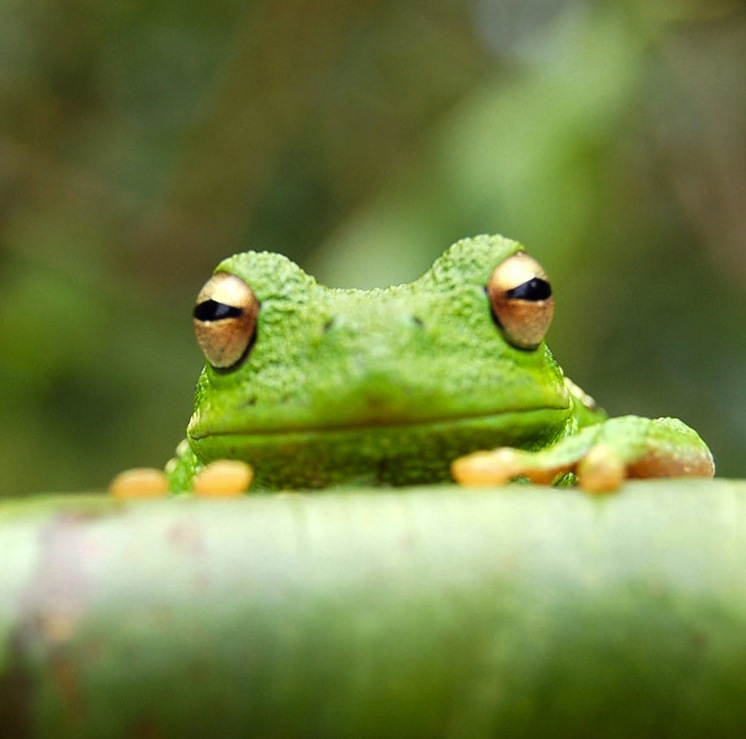
\includegraphics[width=0.2\textwidth]{images/frog.jpg}
    \caption{Illustration d'une grenouille}
    \label{fig:frog1}
\end{figure}

Excepteur sint occaecat cupidatat
non proident, sunt in culpa\ref{fig:frog1} qui officia deserunt mollit anim id est laborum.
Lorem ipsum dolor sit amet, consectetur adipisicing elit, sed do eiusmod tempor incididunt ut
labore et dolore magna aliqua. 

\section{exemple d'insertion d'un tableau}
Lorem ipsum dolor sit amet, consectetur adipisicing elit, sed do eiusmod tempor incididunt ut
labore et dolore magna aliqua. Ut enim ad minim veniam, quis nostrud exercitation ullamco
laboris nisi ut aliquip ex ea commodo consequat. Duis aute irure dolor in reprehenderit in
voluptate velit esse cillum dolore eu fugiat nulla pariatur (ex. Tableau \ref{table:1}). 
\begin{table}[h!]
    \centering
    \begin{tabular}{||c c c c||} 
     \hline
     Col1 & Col2 & Col2 & Col3 \\ [0.5ex] 
     \hline\hline
     1 & 6 & 87837 & 787 \\ 
     2 & 7 & 78 & 5415 \\
     3 & 545 & 778 & 7507 \\
     4 & 545 & 18744 & 7560 \\
     5 & 88 & 788 & 6344 \\ [1ex] 
     \hline
    \end{tabular}
    \caption{Exemple de tableau et de libellé}
    \label{table:1}
\end{table}


Excepteur sint occaecat cupidatat
non proident, sunt in culpa\ref{fig:frog1} qui officia deserunt mollit anim id est laborum.
Lorem ipsum dolor sit amet, consectetur adipisicing elit, sed do eiusmod tempor incididunt ut
labore et dolore magna aliqua. 


\section{Exemple de référence aux acronymes}
Lorem ipsum dolor \ac{MPC} sit amet, consectetur adipisicing elit, sed do eiusmod tempor incididunt ut
labore et dolore magna aliqua. Ut enim ad minim veniam, quis nostrud exercitation ullamco
laboris nisi ut aliquip ex ea commodo consequat. Duis aute irure dolor in reprehenderit in
voluptate velit esse cillum dolore eu fugiat nulla pariatur (ex. Tableau \ref{table:1}). 

  \include{content/chapitre2.tex}
  \include{content/chapitre3.tex}
  \chapter*{Conclusion}
\addcontentsline{toc}{chapter}{Conclusion}
Lorem ipsum dolor sit amet, consectetur adipisicing elit, sed do eiusmod
tempor incididunt ut labore et dolore magna aliqua. Ut enim ad minim veniam,
quis nostrud exercitation ullamco laboris nisi ut aliquip ex ea commodo
consequat. Duis aute irure dolor in reprehenderit in voluptate velit esse
cillum dolore eu fugiat nulla pariatur. Excepteur sint occaecat cupidatat non
proident, sunt in culpa qui officia deserunt mollit anim id est laborum.

Lorem ipsum dolor sit amet, consectetur adipisicing elit, sed do eiusmod
tempor incididunt ut labore et dolore magna aliqua. Ut enim ad minim veniam,
quis nostrud exercitation ullamco laboris nisi ut aliquip ex ea commodo
consequat. Duis aute irure dolor in reprehenderit in voluptate velit esse
cillum dolore eu fugiat nulla pariatur. Excepteur sint occaecat cupidatat non
proident, sunt in culpa qui officia deserunt mollit anim id est laborum.
  \printbibliography 
\addcontentsline{toc}{chapter}{Bibliographie}
  \thispagestyle{empty}
\section*{Acronymes}
\addcontentsline{toc}{chapter}{Liste des acronymes}
\begin{acronym}[AWGN]
	\acro{MPC}{Model Predictive Control}
	\acro{UFR}{Unité de formation et de recherche}
\end{acronym}
  \thispagestyle{empty}
\listoffigures 
\addcontentsline{toc}{chapter}{Table des figures}
\clearpage
\listoftables
\addcontentsline{toc}{chapter}{Table des tableaux}
\newpage
  \include{sides/dernièrePage.tex}
  \thispagestyle{empty}
NANTES UNIVERSITÉ\hfill Année de la soutenance\\
\mbox{}\hfill2023
\vspace{0.5cm}
\Pointilles{1}
\vspace{0.1cm}
\par Nom -- Prénoms~: Nom exemple -- Prénoms exemple\\
Titre de la thèse~: \g{\thetitle} 
\vspace{0.5cm}
\Pointilles{1}
\vspace{0.1cm}
\textbf{Résumé}\\
Lorem ipsum dolor sit amet, consectetur adipisicing elit, sed do eiusmod
tempor incididunt ut labore et dolore magna aliqua. Ut enim ad minim veniam,
quis nostrud exercitation ullamco laboris nisi ut aliquip ex ea commodo
consequat. Duis aute irure dolor in reprehenderit in voluptate velit esse
cillum dolore eu fugiat nulla pariatur. Excepteur sint occaecat cupidatat non
proident, sunt in culpa qui officia deserunt mollit anim id est laborum.

Lorem ipsum dolor sit amet, consectetur adipisicing elit, sed do eiusmod
tempor incididunt ut labore et dolore magna aliqua. Ut enim ad minim veniam,
quis nostrud exercitation ullamco laboris nisi ut aliquip ex ea commodo
consequat. Duis aute irure dolor in reprehenderit in voluptate velit esse
cillum dolore eu fugiat nulla pariatur. Excepteur sint occaecat cupidatat non
proident, sunt in culpa qui officia deserunt mollit anim id est laborum.
\vspace{0.5cm}
\Pointilles{1}
\vspace{0.1cm}
MOTS CLÉS\\
MOT CLÉ 1, MOT CLÉ 2, MOT CLÉ 3, MOT CLÉ 4, MOT CLÉ 5, MOT CLÉ 6.\vfill
\textbf{JURY}\newline
\textbf{Présidente}~: Mme Prénom Nom, Professeur de Virologie, UFR Sciences Pharmaceutiques et Biologiques de Nantes\newline
\textbf{Directeur}~: M Prénom Nom, Professeur de Virologie, UFR Sciences Pharmaceutiques et Biologiques de Nantes\newline
\textbf{Assesseurs}~: M Prénom Nom, Pharmacien d’officine, Nantes
\end{document}